% !TEX TS-program = pdflatex
% !TEX encoding = UTF-8 Unicode

% This is a simple template for a LaTeX document using the "article" class.
% See "book", "report", "letter" for other types of document.


\documentclass[11pt]{article} % use larger type; default would be 10pt

\usepackage[utf8]{inputenc} % set input encoding (not needed with XeLaTeX)

%%% Examples of Article customizations
% These packages are optional, depending whether you want the features they provide.
% See the LaTeX Companion or other references for full information.

%%% PAGE DIMENSIONS
\usepackage{geometry} % to change the page dimensions
\geometry{a4paper} % or letterpaper (US) or a5paper or....
% \geometry{margin=2in} % for example, change the margins to 2 inches all round
% \geometry{landscape} % set up the page for landscape
%   read geometry.pdf for detailed page layout information

\usepackage{graphicx} % support the \includegraphics command and options
\usepackage{subfigure}
\usepackage{pdfpages}

% \usepackage[parfill]{parskip} % Activate to begin paragraphs with an empty line rather than an indent

%%% PACKAGES
\usepackage{booktabs} % for much better looking tables
\usepackage{array} % for better arrays (eg matrices) in maths
\usepackage{paralist} % very flexible & customisable lists (eg. enumerate/itemize, etc.)
\usepackage{verbatim} % adds environment for commenting out blocks of text & for better verbatim
\usepackage{subfig} % make it possible to include more than one captioned figure/table in a single float
% These packages are all incorporated in the memoir class to one degree or another...

%%% HEADERS & FOOTERS
\usepackage{fancyhdr} % This should be set AFTER setting up the page geometry
\pagestyle{fancy} % options: empty , plain , fancy
\renewcommand{\headrulewidth}{0pt} % customise the layout...
\lhead{}\chead{}\rhead{}
\lfoot{}\cfoot{\thepage}\rfoot{}

%%% SECTION TITLE APPEARANCE
\usepackage{sectsty}
\allsectionsfont{\sffamily\mdseries\upshape} % (See the fntguide.pdf for font help)
% (This matches ConTeXt defaults)

%%% ToC (table of contents) APPEARANCE
\usepackage[nottoc,notlof,notlot]{tocbibind} % Put the bibliography in the ToC
\usepackage[titles,subfigure]{tocloft} % Alter the style of the Table of Contents
\renewcommand{\cftsecfont}{\rmfamily\mdseries\upshape}
\renewcommand{\cftsecpagefont}{\rmfamily\mdseries\upshape} % No bold!

%%% END Article customizations

%%% The "real" document content comes below...

\title{Developerhandbuch}
\author{Dominik Otto, 
Lukas Kröger, 
Maximilian Schirm, 
Karsten Schaefers}
%\date{} % Activate to display a given date or no date (if empty),
         % otherwise the current date is printed 

\begin{document}
\maketitle

\section{Zielbestimmung}

\subsection{Client}

\subsubsection{Einführung}
Das Ziel ist es, eine Client-Server-Applikation zur Konvertierung von BibTeX Einträgen unter Berücksichtigung eines .csl-Regelsets in HTML oder Text zu entwerfen.
Dies soll über skalierbare Micro-Services realisiert werden. Die Client-Anfragen werden von einer
Message-Queue verwaltet und auf (einen oder mehrere) Server verteilt.

\subsubsection{Muss-Kriterien}

\begin{itemize}
\item{Das System besteht aus drei (verschiedenen) Komponententypen: Client, Server und Micro-Services}
\item{Der Status der Anfragen in der Message-Queue muss ersichtlich sein}
\item{Auswählen eines .csl-Regelsets, d.h.: eine oder mehrere .csl-Dateien}
\item{Auswählen eines Sets von .bib-Dateien, d.h.: eine oder mehrere .bib-Datei(en)}
\item{Es muss möglich sein Anfragen von mehreren Clients aus zu senden}
\item{Es muss die Möglichkeit bestehen jederzeit neue Anfragen und Übersetzungsservices
hinzuzufügen oder zu entfernen}
\item{Die Übersetzungsservices müssen zusammen eine gewisse Performanz vorweisen (1.000
Anfragen in weniger als 60 Sekunden)}
\end{itemize}

\subsubsection{Wunsch-Kriterien}

\begin{itemize}
\item{Intuitive Bedienung durch ansprechende Client-Benutzeroberfläche (GUI)}
\item{Abspeichern der übersetzten Einträge als Datei}
\item{Optimierung der Übersetzungsperformanz}
\item{Nutzerauthentifizierung}
\item{Status aktuell laufender Anfragen im eigenen Client einsehen}
\end{itemize}

\subsubsection{Abgrenzungskriterien}

\begin{itemize}
\item{Das Programm ist kein Messenger oder ähnliches, d.h.: es besteht keinerlei Möglichkeit zur
Kommunikation unter den Clients.}
\item{Die Übersetzungsservices sind Micro-Services; von daher sollen die Funktionen auf das Nötigste beschränkt werden: Das Übersetzen von BibTeX in HTML oder Text; weitere Funktionen sind nicht gewünscht.}
\end{itemize}

\subsection{Server}

Ein (oder mehrere) Übersetzungsservice(s) laufen auf einem Server und warten auf Anfragen. Das
Annehmen der Übersetzungsanfragen von den Quellen, sowie das Aufteilen auf die
Übersetzungsservices bzw. Server, wird von der Message-Queue bewerkstelligt. Diese ist die
Schnittstelle zwischen Client(s) und Server(n). Die Aufgaben des Servers sind:

\begin{itemize}
\item{Korrekte Übersetzung des gewählten .bib-Sets auf einem oder mehreren Servern
unter Berücksichtigung des gewählten .csl-Regelsets in HTML oder Text}
\item{Die gesendeten Anfragen bearbeiten, übersetzen und anschließend korrekt an die
entsprechenden Clients zurücksenden}
\item{Die Anfragenverwaltung und -verteilung erfolgt durch eine Message-Queue}
\end{itemize}

\subsection{Micro-Service}

Die Micro-Services werden automatisch vom Server angelegt. Sie bekommen von der Message-Queue Anfragen zugewiesen, bearbeiten diese und geben die entsprechenden Ergebnisse zurück. Weitere Funktionen sind nicht gewünscht.

\clearpage

\section{Podukteinsatz}

\subsection{Anwendungsbereich}

Mithilfe des Programms können viele Bibtex-Einträge in  Text oder HTML umgewandelt werden. Dadurch kann zum Einen das Literaturverzeichnis einer Publikation separat veröffentlicht werden. Zum Anderen können noch einzelne Bibtex Einträge zeitsparend umgewandelt werden, um sie zum Beispiel auf einer Website als HTML zu präsentieren.

\subsection{Zielgruppe}

Das Programm kann von Autoren wissenschaftlicher und journalistischer Werke für die in 2.1 genannten Anwendungsmöglichkeiten verwendet werden. Außerdem können auch Verlage Sammlungen ihrer Veröffentlichungen mithilfe der entsprechenden BibTeX-Einträge angeben.


\clearpage

\section{Produktumgebung}

\subsection{Client}

Der Client wird plattformunabhängig in Java entwickelt und läuft deshalb auf allen drei gängigen Endnutzerbetriebssystemen (Windows, Linux, MacOS X). Für die Kommunikation mit dem Server wird entweder eine Internetverbindung benötigt oder der Server muss sich im selben Netzwerk wie der Client befinden.

\subsection{Server}

Die Software für den Server wird ebenfalls in Java entwickelt. Auch dieser muss entweder über eine permanente Internetverbindung verfügen oder sich im selben Netzwerk wie die Clients befinden.

\subsection{Micro-Service}

Der Micro-Service wird, wie die anderen Komponenten auch, in Java implementiert.

\subsection{Produktschnittstellen}

Der Client und der Server müssen in der Lage sein, untereinander zu kommunizieren. Hierfür wird eine Message-Queue mit 'publish-subscribe pattern' verwendet.
Desweiteren müssen Server und Micro-Services miteinander kommunizieren. Dies geschieht ebenfalls nach o.g. Prinzip.

\clearpage

\section{Funktionale Anforderungen}

\subsection{Funktionale Anforderungen an die Client}

\subsubsection{Benutzeroberfläche}

\begin{itemize}
\item{\textbf{/F100/} Benutzer können .csl-Dateien in den aktuellen Auftrag hinzufügen oder entfernen}

\begin{itemize}
\item{\textbf{/F1000/} Die aktuell geladenen .csl-Dateien werden in einer Liste dargestellt}
\item{\textbf{/F1001/} In dieser Liste können Einträge markiert und anschließend über zu der Liste gehörende Controls entfernt werden}
\item{\textbf{/F1002/} Über zu der Liste gehörende Controls können Einträge hinzugefügt werden}

\begin{itemize}
\item{\textbf{/F10020/} Das Hinzufügen erfolgt über einen Dateiwahldialog}
\item{\textbf{/F10021/} Der Dateiwahldialog gestattet lediglich die Auswahl von *.csl Dateien}
\item{\textbf{/F10022/} Wird keine gültige Auswahl getroffen so wird kein Eintrag hinzugefügt}
\item{\textbf{(Optional) /F10023/} Eine ausgewählte Datei ist gültig, wenn ihr Inhalt für eine .csl-Datei korrekt formatiert ist}
\end{itemize}

\end{itemize}

\item{\textbf{/F101/} Benutzer können .bib-Dateien in den aktuellen Auftrag hinzufügen oder entfernen}

\begin{itemize}
\item{\textbf{/F1010/} Die aktuell geladenen .bib-Dateien werden in einer Liste dargestellt}
\item{\textbf{/F1011/} In dieser Liste können Einträge markiert und anschließend über zu der Liste gehörende Controls entfernt werden}
\item{\textbf{/F1012/} Über zu der Liste gehörende Controls können Einträge hinzugefügt werden}

\begin{itemize}
\item{\textbf{/F10120/} Das Hinzufügen erfolgt über einen Dateiwahldialog}
\item{\textbf{/F10121/} Der Dateiwahldialog gestattet lediglich die Auswahl von *.bib Dateien}
\item{\textbf{/F10122/} Wird keine gültige Auswahl getroffen so wird kein Eintrag hinzugefügt}
\item{\textbf{(Optional) /F10123/} Eine ausgewählte Datei ist gültig, wenn ihr Inhalt für eine .bib-Datei korrekt formatiert ist}
\end{itemize}

\end{itemize}

\item{\textbf{/F102/} Benutzer müssen ein Ausgabeverzeichnis wählen bevor ein Auftrag generiert werden kann}

\begin{itemize}
\item{\textbf{/F1020/} Die Auswahl eines Ausgabeverzeichnisses erfolgt mittels eines Verzeichnisbrowsers}
\item{\textbf{/F1021/} Das Gewählte Ausgabeverzeichnis ist auf der Benutzeroberfläche erkenntlich}
\end{itemize}

\end{itemize}

\subsubsection{Serververbindung}

\begin{itemize}
\item{\textbf{/F110/} Benutzer müssen sich zur Konvertierung mit einem Server verbinden. Dazu muss ein Auswahlfenster mit einer Liste von im Netz entdeckten Servern angezeigt werden. Für diesen Vorgang werden /F1101/ bis /F1103/ benötigt. Es können keine Anfragen versandt werden, bis der Client eine gültige Verbindung zu einem Server aufgebaut hat.}

\begin{itemize}
\item{\textbf{/F1101/} Der Nutzer muss die Möglichkeit erhalten, manuell eine Serveradresse festzulegen}
\item{\textbf{/F1102/} Nach Auswahl eines Servers wird der Client am Server authentifiziert (siehe auch /F201/)}
\item{\textbf{/F1103/} Ist die Verbindung mit dem gewählten Server nicht möglich, so wird eine Fehlermeldung angezeigt und der Nutzer kann erneut eine Serverauswahl treffen}
\end{itemize}

\item{\textbf{/F111/} Benutzer können einen aktuell laufenden Konvertierungsauftrag abbrechen}

\begin{itemize}
\item{\textbf{/F1110/} Der Abbruch erfolgt über die Interaktion mit einem Button auf der Oberfläche}
\item{\textbf{/F1111/} Eine Abbruchanfrage wird an den Server versandt}
\end{itemize}

\item{\textbf{/F112/}Benutzer werden benachrichtigt, sobald der Server nicht mehr erreichbar ist}

\item{\textbf{/F113/} Verbindung mit einem anderen Server: Erfolgt durch Eingabe einer neuen Serveradresse und dem Auslösen eines Buttons auf der Oberfläche}

\end{itemize}

\subsubsection{Konvertierungsauftrag}

\begin{itemize}
\item{\textbf{/F120/} Benutzer können einen Konvertierungsauftrag erstellen}

\begin{itemize}
\item{\textbf{/F1200/} Ein Konvertierungsauftrag wird erstellt, wenn die Vorbedingungen (mind. 1 .bib-File, gültige Serververbindung gem. /F110/, kein laufender Auftrag von der gleichen ClientID) erfüllt sind und der Benutzer einen Button auf der Benutzeroberfläche betätigt}
\item{\textbf{/F1201/} Ein gültiger Auftrag wird an den verbundenen Server gesendet}
\item{\textbf{/F1202/} Schlägt der Versand des Auftrags an den Server fehl, so wird dieser erneut versucht bevor dem Benutzer eine Fehlermeldung angezeigt wird}
\item{\textbf{/F1203/} Läuft ein Auftrag, ist es nicht möglich einen weiteren zu versenden, bevor der aktuelle "abgebrochen", "fehlgeschlagen" oder "fertiggestellt" ist}
\end{itemize}

\item{\textbf{/F121/} Ein Konvertierungsauftrag wird als codiertes Objekt über Netzwerk an den Server übermittelt}

\begin{itemize}
\item{\textbf{/F1210/} .bib-Dateien werden vor der Codierung in BibTeX-Einträge eingeteilt und anschließend in einer Liste verwaltet, .csl-Dateien werden den eben genannten Einträgen zugeordnet}
\item{\textbf{/F1212/} Ein Auftrag enthält eine Liste von BibTeX-Einträgen}
\item{\textbf{/F1213/} Ein Auftrag enthält die ID des Clients}
\item{\textbf{/F1214/} Die Informationen des Auftrags werden als einzelnes Objekt an den Server übermittelt}
\end{itemize}

\item{\textbf{/F122/} Erhält der Client eine gültige Bestätigungsnachricht vom Server, so werden die in dieser Nachricht codierten Dateien in das Ausgabeverzeichnis decodiert (und  /F1123/)}

\end{itemize}

\subsection{Funktionale Anforderungen an den Server}

\subsubsection{Kommunikation}

\begin{itemize}
\item{\textbf{/F200/} Der Server wartet auf einem festgelegten Port auf Verbindungsanfragen von Clients}
\item{\textbf{/F201/} Trifft eine Verbindungsanfrage ein, so wird ein Authentifizierungsverfahren durchgeführt}

\item{\textbf{/F202/} Trifft ein Konvertierungsauftrag mit gültiger Client ID ein, wird dieser angenommen}

\begin{itemize}
\item{\textbf{/F2020/} Ist auf dem Server noch ein laufender Auftrag für diese Client ID hinterlegt, so wird dieser abgebrochen}
\item{\textbf{(Optional) /F2021/} Der Auftrag wird nach seinem Umfang bewertet und entsprechend priorisiert (vgl. /F211/)}
\item{\textbf{/F2022/} Für den Auftrag wird ggf. ein neuer Service gestartet und diesem der Auftrag übergeben}
\end{itemize}

\item{\textbf{/F203/} Trifft eine Abbruchanfrage mit gültiger Client ID ein wird eine Abbruchanfrage an den zugeordneten Server versandt}
\item{\textbf{/F204/} Wird der Server beendet, so wird eine Abbruchnachricht an alle laufenden Services versandt und die momentan wartenden Clients erhalten Statusmeldungen mit Fehler}
\end{itemize}

\subsubsection{Funktionalität}

\begin{itemize}
\item{\textbf{/F210/} Der Server kann Konvertierungsaufträgen lesen}
\item{\textbf{(Optional) /F211/} Der Server priorisiert Aufträge nach Umfang}
\item{\textbf{/F212/} Der Server verwaltet Services}

\begin{itemize}
\item{\textbf{/F2120/} Der Server kann Services starten}
\item{\textbf{/F2121/} Der Server kann Services durch Abbruchanfragen vorzeitig beenden}
\item{\textbf{/F2123/} Der Server vergibt Aufträge an Services}
\end{itemize}

\item{\textbf{/F213/} Pro Plattform kann nur eine Instanz des Servers ausgeführt werden}
\item{\textbf{/F214/} Ist der festgelegte Port des Servers bei Start belegt kann der Server nicht gestartet werden und eine Fehlermeldung wird angezeigt}
\end{itemize}

\subsubsection{(Optional) GUI}

\begin{itemize}
\item{\textbf{/F220/} Der Server zeigt eine Liste der aktuell registrierten Clients}

\begin{itemize}
\item{\textbf{/F2200/} Über Controls neben der Liste können Clients gesperrt werden}
\end{itemize}

\item{\textbf{/F221/} Der Server zeigt eine Liste der aktuell registrierten Aufträge}

\begin{itemize}
\item{\textbf{/F2210/} Über Controls neben der Liste können Aufträge abgebrochen}
\end{itemize}

\item{\textbf{/F222/} Der Server zeigt eine Liste der aktuell registrierten Services}

\begin{itemize}
\item{\textbf{/F2220/} Über Controls neben der Liste können Services abgebrochen werden}
\end{itemize}

\item{\textbf{/F223/} Der Server kann über einen Button beendet werden}
\end{itemize}

\subsection{Funktionale Anforderungen an Services}

\subsubsection{Funktionalität}

\begin{itemize}
\item{\textbf{/F300/} Services kombinieren .bib und .csl-Dateien und konvertieren sie zu HTML oder Text}

\begin{itemize}
\item{\textbf{/F3000/} Services akzeptieren für die Konvertierung mehrere BIB und mehrere CSL Dateien}
\end{itemize}

\item{\textbf{/F301/} Jeder Service läuft in einem eigenen Prozess}
\item{\textbf{/F302/} Der Service muss sich ein eigenes Arbeitsverzeichnis erstellen und dieses selbstständig verwalten}

\begin{itemize}
\item{\textbf{/F3020/} Nach Beendigung einer Konvertierung oder Beendigung eines Services muss das Verzeichnis gelöscht werden}
\end{itemize}

\end{itemize}

\subsubsection{Kommunikation}

\begin{itemize}
\item{\textbf{/F310/} Nach der Beendigung der Konvertierung eines Auftrags (/F300/ ff.) werden die Ergebnisdateien (HTML/Text) codiert und an den Auftraggeber versandt}
\item{\textbf{/F311/} Trifft eine Abbruchanfrage von dem Auftraggeber ein, so wird die aktuell laufende Operation abgebrochen}
\end{itemize}

\clearpage

\section{Produktdaten}

\subsection{Client}

\begin{itemize}
\item[\textbf{/P01/} .bib-Dateien]{\ \\Der Client muss die zu konvertierenden \.bib-Dateien vorliegen haben, um sie gemäß /F101/ zu einem Auftrag hinzuzufügen und per /F3000/ an den Server zu übertragen}
\item[\textbf{/P02/} CSL-Dateien]{\ \\Der Client muss die für die Konvertierung notwendigen CSL-Dateien vorliegen haben, um sie gemäß /F100/ zu einem Auftrag hinzuzufügen und per /F3000/ an den Server zu übertragen}
\end{itemize}

\clearpage

\section{Nichtfunktionale Anforderungen}

Neben den genannten funktionalen Anforderungen, werden an die zu entwickelnde Applikation auch diverse nichtfunktionale Anforderungen gestellt, die sich leicht zu den folgenden Kategorien zuordnen lassen.

\subsection{Bedienung}

\textbf{/N010/} Das Programm soll eine eingängige und simple Bedienung ermöglichen. Darunter ist zum Einen zu verstehen, dass der Endnutzer nicht mit jedweden Anfragen behelligt werden soll, welche technisches Vorwissen erfordern. Zum Anderen sollen die Möglichkeiten, die die Applikation bietet, übersichtlich dargestellt sein, sodass dem Endnutzer stets alle Optionen zur Verfügung stehen.

\subsection{Sicherheit}

\textbf{/N020/} Das Programm soll grundlegende Sicherheitsfunktionen erfüllen. Darunter fällt, dass die zu übermittelnden Daten an den Server nicht im Klartext übermittelt werden, was auch für die Antworten des Servers an den Client gilt.
\subsection{Erreichbarkeit}

\textbf{/N030/} Der Server, auf dem das Programm arbeitet sollte möglichst stets erreichbar sein. Falls dies einmal nicht der Fall ist, so soll die Applikation dies erkennen und den Endnutzer mit entsprechendem Dialog darauf hinweisen. Eine optionale Anforderung ist die Möglichkeit, das Programm auch ohne erreichbaren Server mit begrenzten Kapazitäten lokal auszuführen.

\subsection{Implementierungseinschränkungen}

\textbf{/N040/} Das Programm (alle 3 Komponententypen) soll mit Java erstellt werden und mindestens auf Linux-Systemen ausführbar sein.

\subsection{Performanz}

\textbf{/N040/} Die Software soll mindestens 1000 Anfragen in weniger als 60 Sekunden bearbeiten können.

\clearpage

\section{Anhang: Diagramme}

\begin{figure}
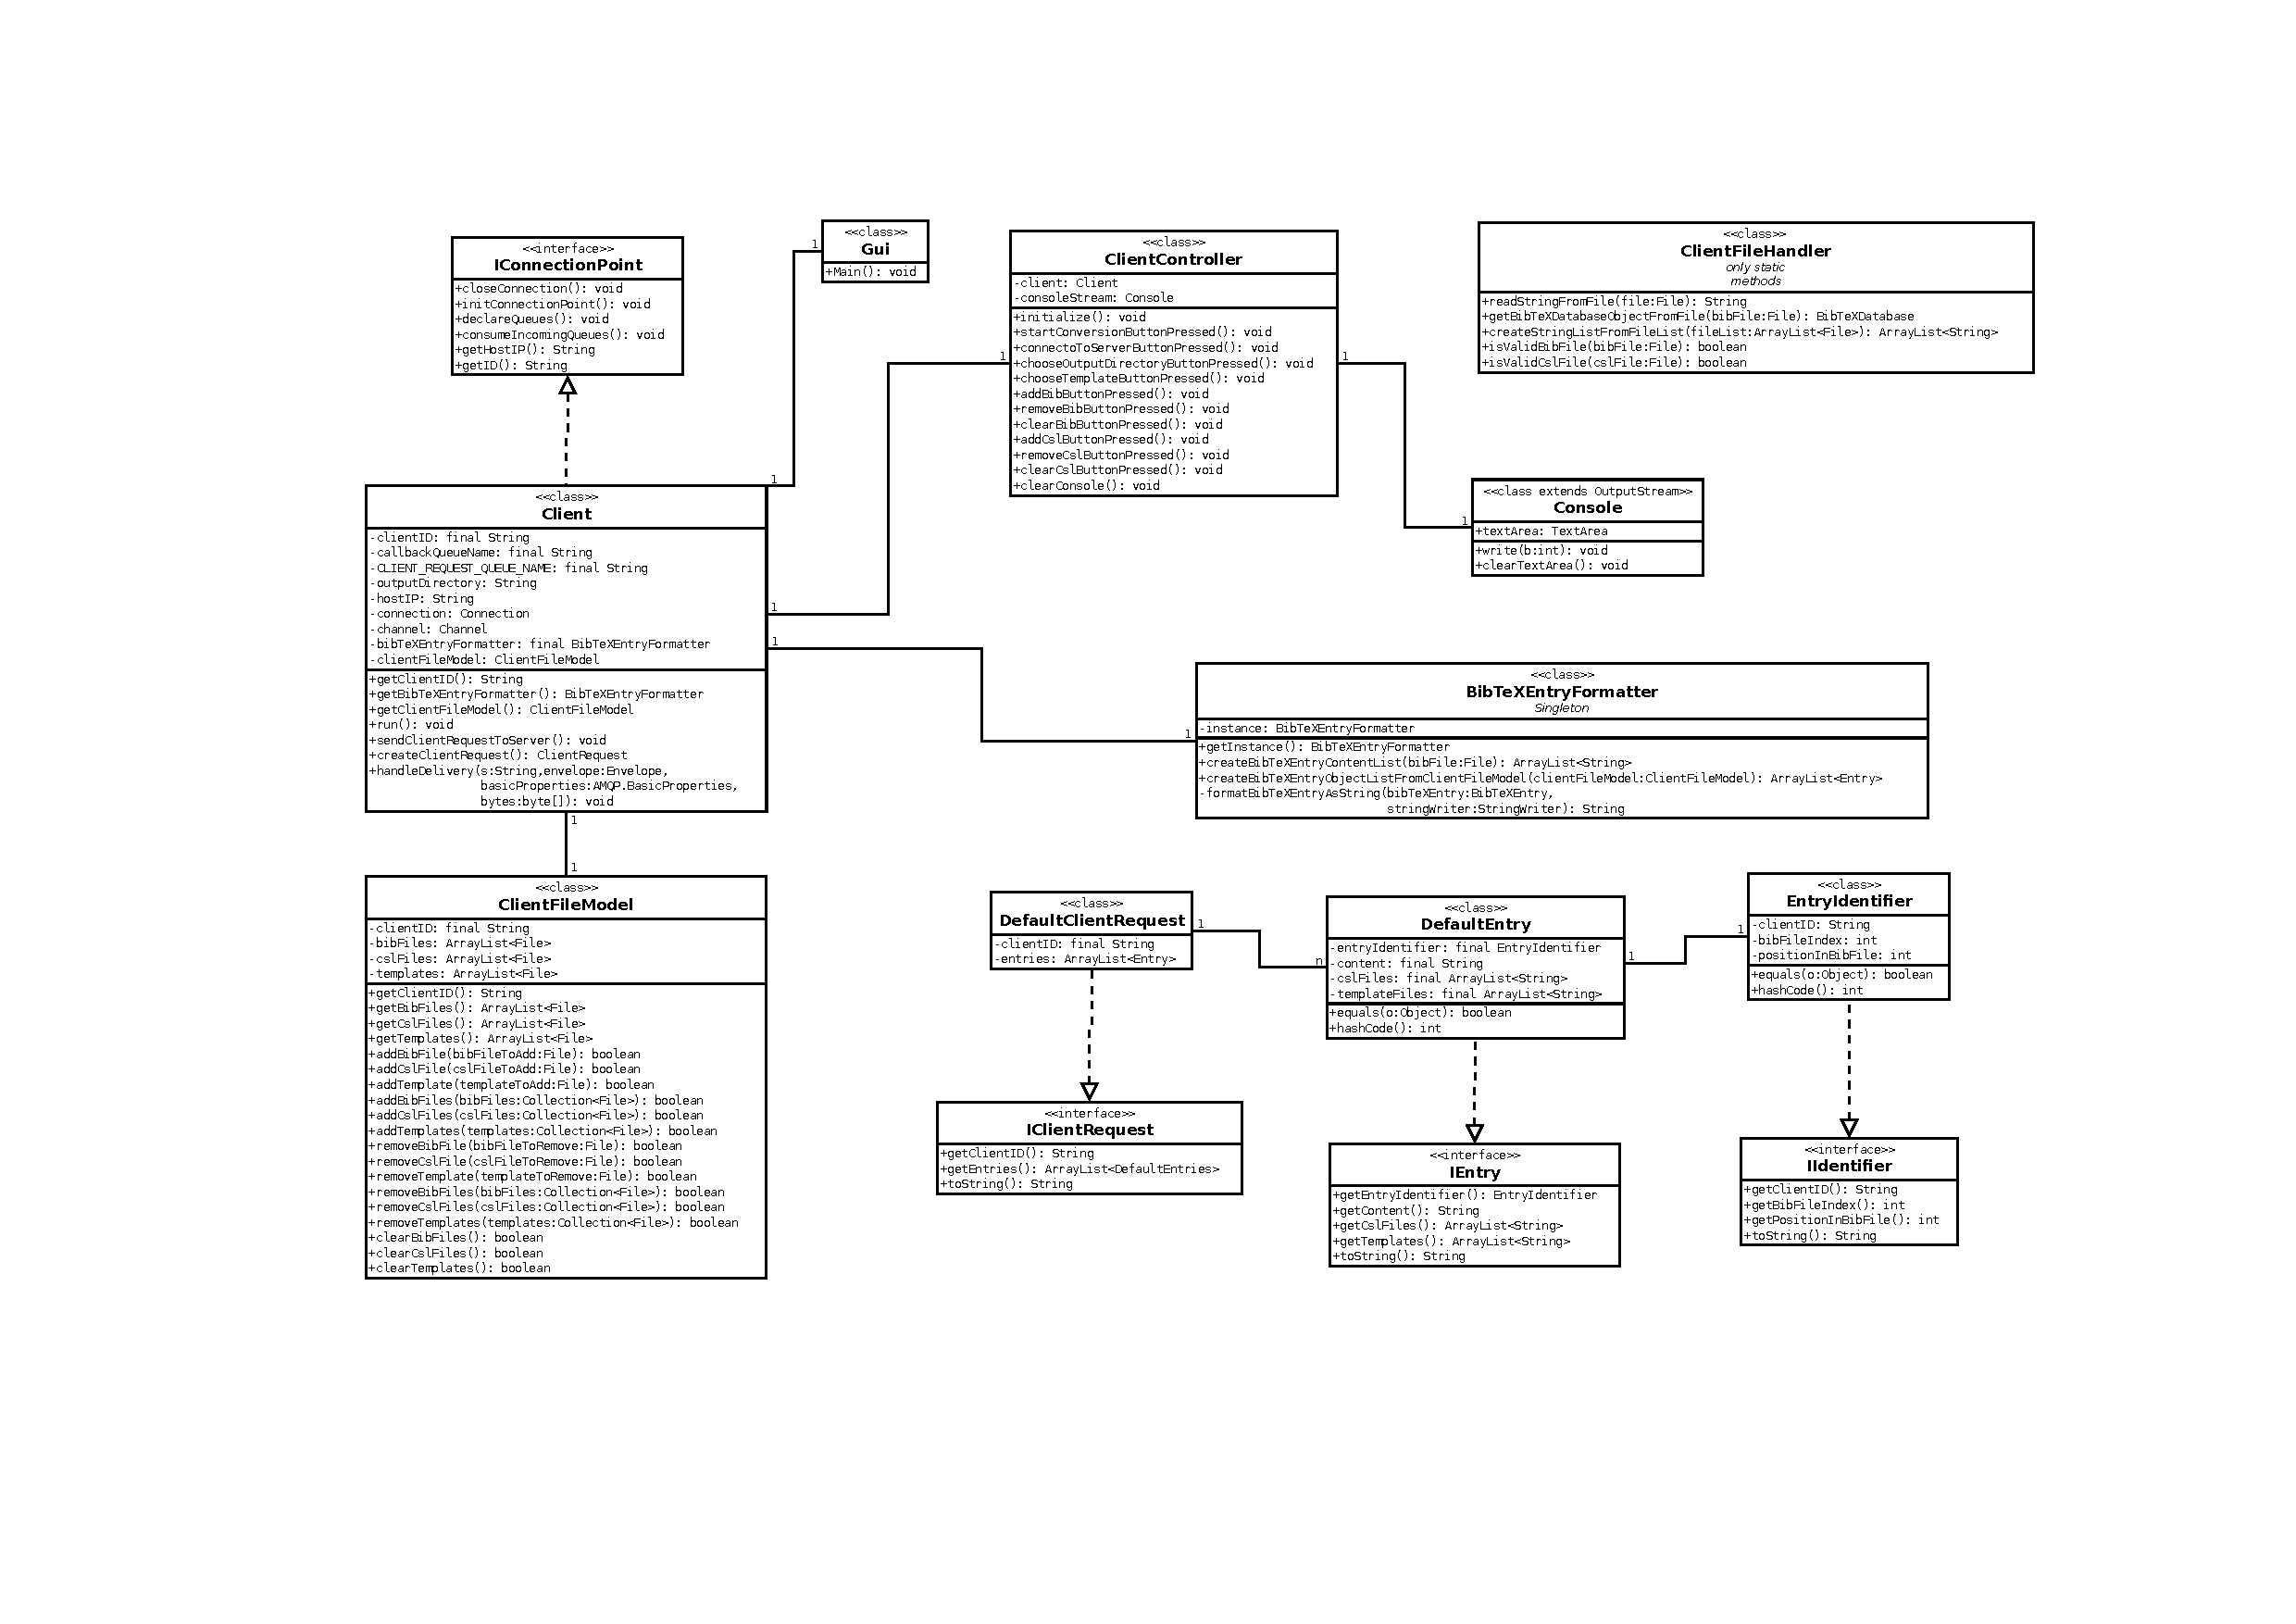
\includepdf{Graphics/Client.pdf}
\end{figure}

\end{document}
